\documentclass{article}
\usepackage{url}
\usepackage{amssymb,amsfonts,amsmath,amsthm,mathtools}
\usepackage{adjustbox}
\usepackage{float}
\usepackage{caption}
\usepackage{mdframed}
\usepackage{lmodern}
\usepackage{bm,bbold}
\usepackage{xfrac, nicefrac}
\usepackage{lmodern}
\usepackage{enumitem}
\usepackage[margin=60pt]{geometry}
\pdfinclusioncopyfonts=1
\captionsetup{width=0.85\textwidth}
\usepackage{pgfplots, pgf,tikz}
\usepgfplotslibrary{fillbetween}
\pdfinclusioncopyfonts=1
\captionsetup{width=0.85\textwidth}

\usepackage{xcolor}
\definecolor{RED}{HTML}{EB6231}
\definecolor{YELLOW}{HTML}{E29D26}
\definecolor{BLUE}{HTML}{5D80B4}
\definecolor{LIGHTGREEN}{HTML}{6ABD9B}
\definecolor{GREEN}{HTML}{8FB03E}
\definecolor{PURPLE}{HTML}{BE1E2D}
\definecolor{BROWN}{HTML}{A97C50}
\definecolor{PINK}{HTML}{DA1C5C}

\newcommand{\specialcell}[2][c]{%
	\begin{tabular}[#1]{@{}c@{}}#2\end{tabular}}

\DeclareMathOperator{\E}{\mathbb{E}}
\newcommand{\der}{\mathrm{d}}
\newcommand{\e}{\mathrm{e}}
\newcommand{\angstrom}{\text{\normalfont\AA}}

% Time, effective population size and mutation rate.
\newcommand{\Ne}{N_{\mathrm{e}}}
\newcommand{\dnds}{\omega}
\newcommand{\Nsite}{\text{n}}
\newcommand{\Nsites}{\text{n}}
\newcommand{\site}{\text{i}}
\newcommand{\Nstate}{\text{K}}

\newcommand{\x}{x}
\newcommand{\eq}{^{*}}
\newcommand{\dx}{\delta \x}
\newcommand{\s}{s}
\newcommand{\deltaG}{\Delta G}
\newcommand{\deltaGMin}{\alpha}
\newcommand{\deltadeltaG}{\Delta \deltaG}

\newcommand{\ci}{\mathbb{S}_{t}}
\newcommand{\cj}{\mathbb{S}_{t}'}
\newcommand{\itoj}{\ci, \cj}
\newcommand{\setNeighbors}{\mathcal{M}\left(\ci\right)}
\newcommand{\setNonSynNeighbors}{\mathcal{N}\left(\ci\right)}
\newcommand{\setSynNeighbors}{\mathcal{S}\left(\ci\right)}
\newcommand{\submatrix}{q}

\begin{document}
\title{Substitution rate responses to changes in effective population size.}
\author{T. Latrille, N. Lartillot}
\maketitle
 
\abstract{
The quasi-neutral theory of evolution asserts that the effective population size ($\Ne$) plays an important role in shaping the evolution of molecular sequences.
One consequence is that $\Ne$ modulates selection, such populations with high $\Ne$ would have stronger purifying selection, due to the decrease of random drift.
In molecular sequence, this effect translates in the decrease in the substitution rate of selected mutations relative to the substitution rate of neutral mutation ($\dnds$) with respect to $\Ne$.
Such theoretical prediction had been observed in empirical data across many clades.
However, several studies failed to observe such response of $\dnds$ to changes in $\Ne$, or with weak strength or direction.
Computational models of protein folding have observed that $\dnds$ can be independent of $\Ne$, which can mathematically be proven under certain assumptions.
Moreover, non-equilibrium properties can imply that an increase of $\Ne$ can result first in an increase of $\dnds$ and then a decrease.
Together, assumptions about the mapping of sequence to fitness can display a variety of behaviors in the $\dnds$ responses to changes in $\Ne$.
Our goal in this present work is to provide theoretical tools to derive the relationship between $\Ne$ and $\dnds$ in the context of a genotype-phenotype-fitness map.
We apply our framework in the special case of fitness proportional to the probability of protein folding.
Our compact theoretical results are supported by more complex simulations using 3d structure of proteins.
We assert that models based on the probability of folding are at odds with empirically results obtained on the $\Ne$-$\dnds$ relationship in population genetic dataset.
However, our framework applied to the case of non-specific interactions between proteins suits more the empirical data.
We also stress the importance of epistatic interactions in the $\Ne$-$\dnds$ relationship, such that it determines to time to reach a new equilibrium, and that models without epistasis might be too slow to be realistic.
}
\section*{Introduction}
Differences in DNA sequences of a gene in separate species are due to the particular history of DNA substitutions along each specie's respective lineage.
These substitutions at the level of the population are the result of point mutations at the level of individuals, subject to evolutionary forces such as selection and random drift.
In protein-coding DNA sequences, non-synonymous mutations are changing the amino-acid sequence, and by comparing the non-synonymous substitutions rate relative to the synonymous substitution rate (supposedly neutral), a statistic called $\dnds$, we can estimate the global strength of selection and random drift.\\
For a given gene, it has been empirically observed changes of $\dnds$ along lineages of a phylogeny \cite{Yang2001, Zhang2004}.
More importantly, changes in substitution rate correlate with changes in life-history-traits (longevity, body mass, ...) such as shown by the molecular comparative framework \cite{Lartillot2011,Weber2014}.
Such covariations are compatible with the theoretical prediction of the nearly neutral theory of evolution \cite{Ohta1972, Ohta1992}, where the underlying mechanism is changes in effective population size ($\Ne$).
Indeed, populations with low $\Ne$ would have both a large body size and a high $\dnds$ (weaker selection) due to the increase of random drift.
If $\dnds$ is empirically correlated to life-history traits, such as body mass and longevity, the direction of correlation could not be replicated across all experiments \cite{Figuet2016}.\\
Theoretical prediction of $\dnds$ decreasing as a function of $\Ne$ had been developed in the context of a fixed distribution of fitness effects of novel mutations \cite{Ohta1972, Welch2008}. Similarly, it has been shown in context of a fixed fitness landscape, where each amino-acid have different fitness \cite{Spielman2015a, DosReis2015}, although sites are considered independently evolving, without epistasis.
Unexpectedly, it has also been argued that the existence of a $\dnds$ response to $\Ne$ is not straightforward, even in the context of nearly neutral theory of evolution \cite{Lanfear2014}.
In the example of a biochemical mechanistic computational model, where the fitness is determined by the probability of folding, $\dnds$ as been observed to be independent of $\Ne$ \cite{Goldstein2013}.
Theoretically, a more general case is obtained whenever the fitness is a concave function of a trait, and such trait is equimutable \cite{Cherry1998}.
Equimutabibilty meaning a mutation has the same effect on the trait whatever the current trait of the individual.
In addition to this complexity, $\dnds$ response to $\Ne$ can be non-monotonic due to non-equilibrium properties, such that an increase in $\Ne$ implies firstly a burst of $\dnds$ (adaptive selection), and subsequently a decrease in $\dnds$ (purifying selection) \cite{Jones2016}.\\
Our goal in this present work to reconcile empirical observation with theoretical results, such as to delimit which models and assumptions are reasonable.
This question is important if we want to extract changes in effective population size from substitution history, as well as to determine the fitness landscape under which protein-coding DNA sequences are evolving.
We provide theoretical tools to derive the relationship between $\Ne$ and $\dnds$ in the context of a genotype-phenotype-fitness map.
We apply our framework in the special case of fitness proportional to the probability of protein folding.
Our compact theoretical results are supported by more complex simulations using 3d structure of proteins.
We assert that models based on the probability of folding are at odds with empirically results obtained on the $\Ne$-$\dnds$ relationship in population genetic dataset.
However, our framework applied to the case of non-specific interactions between proteins suits more the empirical data.
We also stress the importance of epistatic interactions in the $\Ne$-$\dnds$ relationship, such that it determines to time to reach a new equilibrium, and that models without epistasis might be too slow to be realistic.
\section*{Results}
\subsection*{Theoretical approximations}
In this section we theoretically approximate the change in $\dnds$ at equilibrium after a change in $\Ne$, under a model in which the fitness depends on the genotype of the whole sequence.
Firstly, we decompose the map from genotype to fitness through an intermediary bounded phenotype $0 \leq \x \leq 1$, the proportion of unstable sites in the sequence.
Each site of the sequence ($\Nsite$ sites) can be in one of $\Nstate \geq 2$ states, where only $1$ of those states is assumed to be a stable state, and $\Nstate - 1$ states are unstable.
The optimal phenotype is obtained when all of the $\Nsite$ sites of the sequence are stable ($\x = 0$).\\
To complete the model, the phenotype-fitness map is first considered generally, where the Wrightian fitness of phenotype $\x$ is $f(\x)$.
After a mutation, given that only one site can change at a time, the absolute change of $\x$ is either $0$ or $\dx=\sfrac{1}{\Nsite}$.
Most importantly the probabilities to increase or decrease $\x$ are different, and depends on the current phenotype $\x$.
Mutation increasing $\x$ are selected against, while mutations decreasing $\x$ are positively selected. 
Mutation and selection cancel each other at equilibrium, where the expectation of fitness effects of mutations reaching fixation in the population is $0$.
Altogether, the equilibrium phenotype obtained for such mutation-selection balance is denoted $\x\eq$, and more importantly is given by the equation (See Supplementary Materials):
\begin{align}
\ln \left( \frac{1 - \x\eq}{\x\eq} \right) + \ln (\Nstate-1) \simeq - \frac{4\Ne}{\Nsite} \frac{ \partial \ln f(\x\eq) }{\partial {\x\eq}}.
\end{align}
This equation of equilibrium phenotype can be further studied to derive the response of $\x\eq$ after a change in $\Ne$, using differential calculus.
Furthemore, assuming that the number of states is large (typically $20$ for amino-acid), we obtain the change in $\omega\eq$ after a change in $\Ne$ as: 
\begin{align}
\frac{ \der \omega\eq}{\der \ln (\Ne)} & \simeq - \frac{\frac{ \partial \ln f(\x\eq) }{\partial {\x\eq}}}{\frac{ \partial^2 \ln f(\x\eq) }{\partial {\x\eq}^2}}.
\end{align}
In other words, the slope of the $\dnds$ elasticity to changes in $\Ne$ (in log scale) is the ratio of first to the second derivative of the log-fitness function, taken at the equilibrium phenotype. To note, this elasticity is strictly negative for decreasing log-concave fitness functions.\\
So far, our result did not assume any particular parametrization of the phenotype-fitness map.
As an example, already proposed in the literature \cite{Goldstein2011}, fitness is proportional to the probability of our protein to be in the folded state, given by Fermi Dirac distribution: 
\begin{equation}
f(\x) \propto \dfrac{1}{1 + e^{\beta (\deltaGMin + \Nsite \gamma \x)}}, 
\end{equation}
where $\deltaGMin < 0$ and $\gamma > 0$ are in kcal/mol, and the fixed parameter $\beta$ is $1.686$ mol/kcal at room temperature. In other words, $\deltaGMin$ is the difference in free energy between folded and unfolded state when all sites are stable. $\gamma$ is the expected change in free energy (between folded and unfolded states) for a destabilizing mutation.
With such fitness function, the equilibrium phenotype $\x\eq$ is given by the equation: 
\begin{align}
\ln \left( \frac{1 - \x\eq}{\x\eq} \right) + \ln (\Nstate-1) \simeq 4\Ne \beta \gamma e^{\beta (\deltaGMin + \Nsite \gamma \x\eq)}.
\label{eq:equilibrium}
\end{align}
The $\dnds$ elasticity to changes in $\Ne$ simplify to a compact equation: 
\begin{equation}
\frac{ \der \omega\eq}{\der \ln (\Ne)} \simeq -\dfrac{1}{\beta \Nsite \gamma};
\end{equation}
which is independent of $\x\eq$, meaning $\omega$ is linearly decreasing with $\Ne$ in log space.
Moreover, only the free compound parameter $\gamma \Nsite$ has an impact on the slope, an intuition for such result is given in figure \ref{fig:NeChangeInfluence}.
Meaning that under empirically relevant value of $\Nsite=300$ sites and $\gamma=1.0$ kcal/mol \cite{Zeldovich2007}, the slope of the linear relationship between $\dnds$ and log-$\Ne$ is approximately $0.002$.
\begin{figure*}[htb!]
 \begin{mdframed}
  \centering
  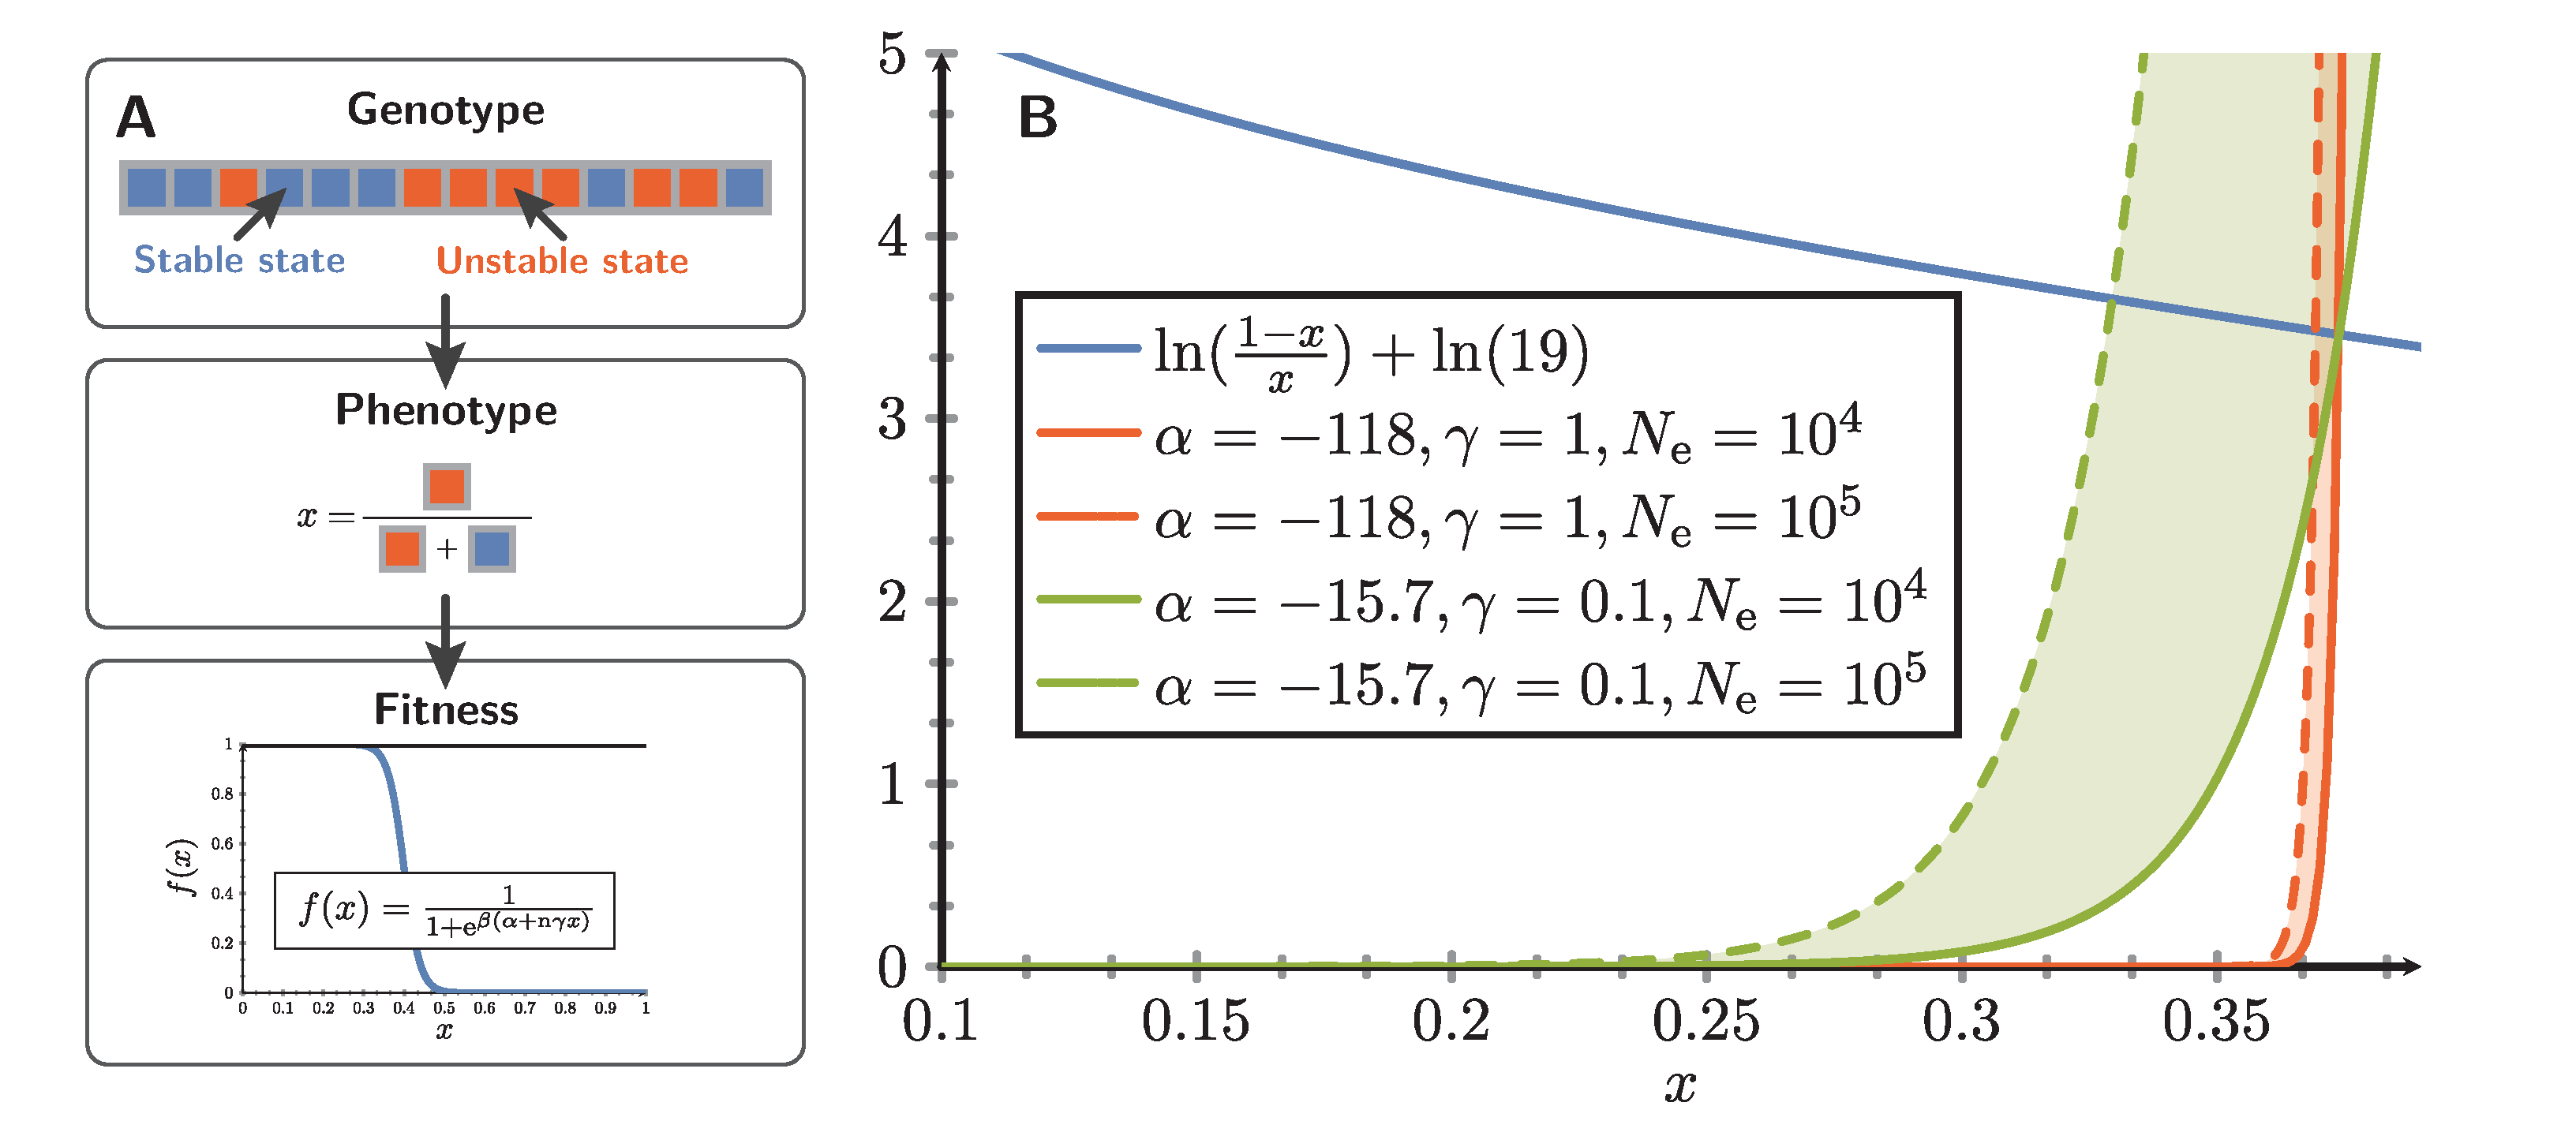
\includegraphics[width=0.9\textwidth, page=1] {artworks/theoretical.pdf}
  \caption{
   \textbf{Theoretical model.}
   Panel A. Illustration of the Genotype-phenotype-fitness map. The phenotype ($\x$) is a real-valued summary of the genotype, and is defined in our model as the fraction of unstable sites in the sequence. The fitness is a decreasing log-concave function of the phenotype.
   Panel B. Illustration of the $\dnds$ elasticity after a change in $\Ne$.
   For the special case $K=2$, the equilibrium $\x\eq$ is determined by the equation $\ln(\frac{1 - \x\eq}{\x\eq})=4\Ne \beta \gamma e^{\beta (\deltaGMin + \Nsite \gamma \x\eq)}$. The right-hand side of the equation increases exponentially with $\x$ where $\Nsite \gamma$ is the exponential growth rate. Thus when $\Nsite \gamma$ is large (red solid line), increasing $\Ne$ (red dotted line) only moves slightly $\x\eq$ (x-axis of the crossing with the blue solid line). On the other hand, when $\Nsite \gamma$ is low (green solid line), increasing $\Ne$ (green dotted line) moves $\x\eq$ notably. Moreover, changes in $\x\eq$ reflects the changes in $\dnds\eq$ since both are related by a monotonous function (See Supplementary Materials). The value of $\alpha$ has been chosen given all other parameters such that the solid lines all cross at the same point.
  }
  \label{fig:NeChangeInfluence}
 \end{mdframed}
\end{figure*}

\subsection*{Simulations confirmation}
Our compact theoretical results are based on assumptions that are broken in practice, for example assuming that 
\begin{enumerate}
 \item $\Nsite$ is large;
 \item selection coefficient is well approximated by the fitness derivative;
 \item genetic code is not taken into account;
 \item all unstable states are equivalently unstable.
\end{enumerate}
We thus first tested the soundness of our theoretical results when such assumptions are relaxed, by simulating DNA sequences evolution (See Methods). 
Firstly, simulations demonstrate that the relation between $\dnds$ and log-$\Ne$ is linear, and that the slope of the linear regression match the expected theoretical value (See Figure \ref{fig:GoldsteinVsToy}).
Secondly the parameter $\deltaGMin$ hardly changes the slope of the linear regression, as expected also theoretically.
Decreasing $\deltaGMin$ (to more negative values) increases $\dnds$, by shifting the equilibrium to higher $\x\eq$ since more unstable sites are fixed before reaching sensible deleterious selection coefficient against unstable mutations. Once many sites are unstable, the $\dnds$ is higher since non-synonymous mutations between unstable states are effectively neutral. However the slope of the $\dnds$-$\Ne$ relationship is not changed, a predicted in our theoretical model.\\

Finally, we compare our results to more complex models of sequence evolution leveraging the $3$D structure of protein \cite{Williams2006, Goldstein2011, Pollock2012}.
In such models, the free energy of the folded state is computed using the $3$D folded structure and pairwise contact potential energies between neighboring amino-acid residues \cite{Miyazawa1985}.
The free energy distribution of unfolded states is approximated using $55$ decoy $3$D structures that supposedly represent a sample of possible unfolded states (see Supplementary Materials).
The original works claimed that under such $3$D model $\dnds$ is independent of $\Ne$.
Using extensive simulations, we argue instead that $\dnds$ is approximately linear with log-$\Ne$ (see Figure \ref{fig:GoldsteinVsToy}, panel C).
Moreover, the observed slope match the theoretical value considering $\deltadeltaG = 1.0$ kcal/mol for destabilizing mutations and $\Nsite=300$. 
In such experiment, $\alpha=-118$ kcal/mol as it is the $\deltaG$ of the most stable sequence of $300$ sites \cite{Goldstein2011}.
\begin{figure*}[htb!]
\begin{mdframed}
\centering
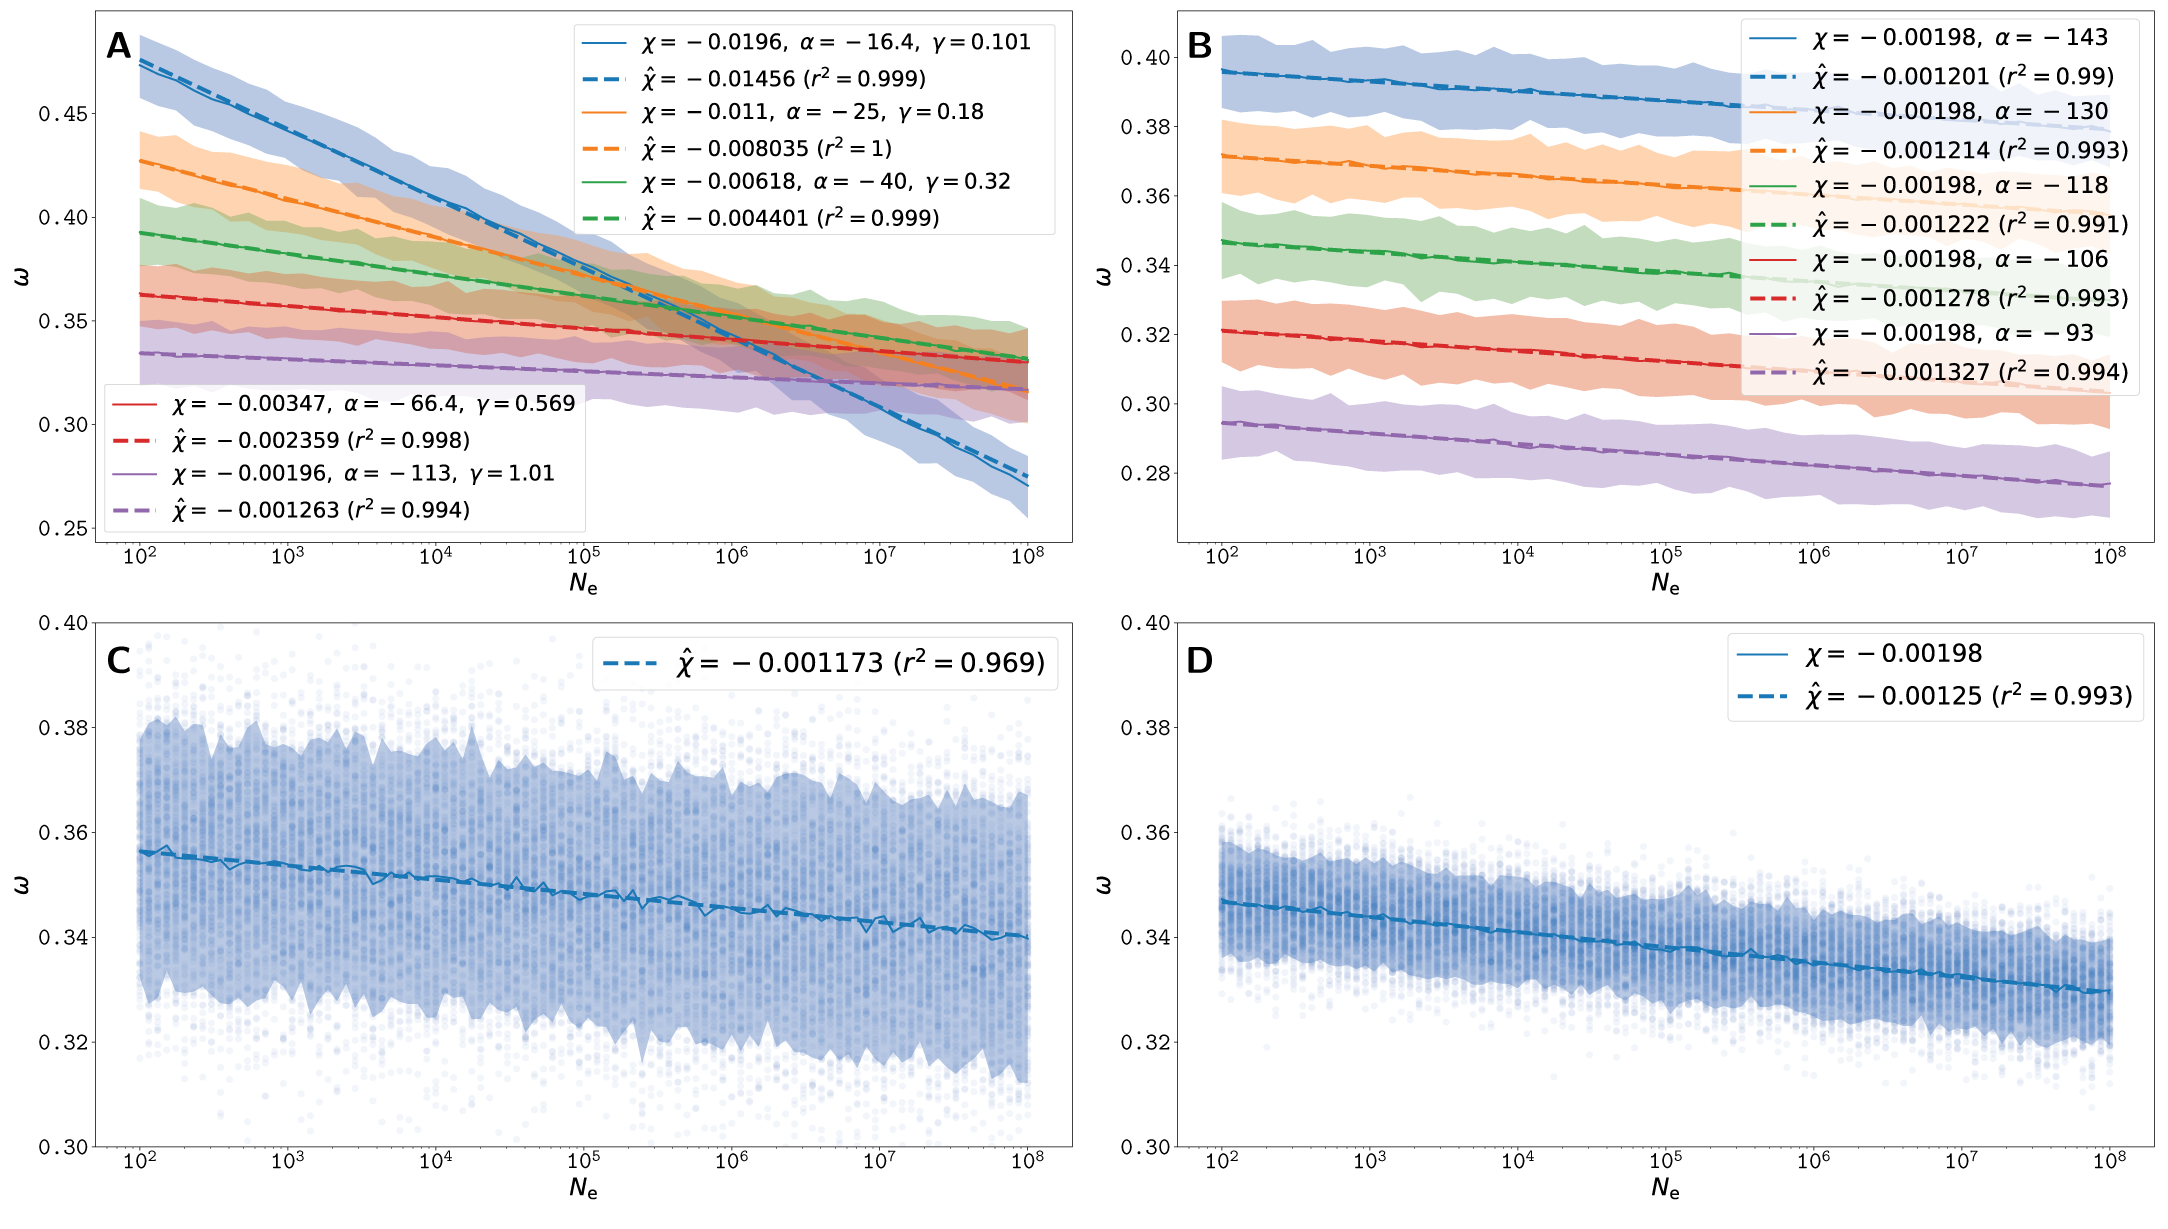
\includegraphics[width=0.9\textwidth] {artworks/Elasticity.png}
 \caption{
  \textbf{$\bm{\dnds}$ elasticity to change in $\bm{\Ne}$}.
  For each population size, $100$ simulations were performed and the average (solid line) and $90\%$ confidence interval (shaded area) are shown.
  Panel A. The fixed parameters are $\gamma=1$, $\Nsite=300$, $\beta=1.686$, and for each non-optimal amino-acid, $\gamma$ is scaled by the Grantham distance to the optimal amino-acid. $\alpha$ are given in the legend. Decreasing $\alpha$ (to more negative values) increases $\dnds$ but changes hardly the slope of the linear regression, as expected theoretically.
  $\dnds$ at equilibrium as a function of $\bm{\Ne}$ (log scale).
  Panel B. The fixed parameters are $\Nsite=300$ and $\beta=1.686$. Parameters $\alpha$ and $\gamma$ are given in the legend.
  $\gamma$ is increased and $\alpha$ is changed accordingly such that the equilibrium value $\x\eq$ is kept constant, by solving numerically equation \ref{eq:equilibrium}.
  The slope of $\dnds$-$\Ne$ relationship decreases proportionally to the inverse of $\gamma$, as predicted by our theoretical model.
  Panel C. In the model of 3D free energy of folding, $\dnds$ at equilibrium is weakly dependent on log-$\Ne$ but is not independent as claimed originally \cite{Goldstein2013}.
  This weak dependence matches the theoretical prediction of our additive free energy model that the linear relation (dashed line) has a slope equal to $(\beta \Nsite \gamma)^{-1} = 0.00198 \simeq 0.00124$.
  Bottom D, the fixed parameters are $\alpha=-118$, $\gamma=1$, $\Nsite=300$, $\beta=1.686$, and for each non-optimal amino-acid, $\gamma$ is scaled by the Grantham distance to the optimal amino-acid.
  Moreover, with the Grantham model, the $\dnds$ matches the empirical 3D model of Golstein \& Pollock and the theoretical prediction.
  \label{fig:GoldsteinVsToy}
 }
\end{mdframed}
\end{figure*}
\subsection*{Epistasis determines the time to relaxation}
Although the equilibrium value of $\dnds$ after changes in $\Ne$ is an important feature of the $\dnds$-$\Ne$ relationship, another parameter that is scarcely studied is the relaxation time to reach the new equilibrium $\dnds$ \cite{Jones2016}.
We observed in our simulations that the determining factor of the relaxation time is the number of sites $\Nsite$ (See Figure \ref{fig:relaxStability}).
Such observations match the theoretical prediction that high epistasis leads to faster return to equilibrium, since more opportunities are available.
In the case of a fitness landscape with epistasis, after a change in $\Ne$, any site that is used to climb either up or down the fitness landscape will have diminishing return in other sites of the sequences.
Not taking into account epistasis have the consequence of overestimating the relaxation time to return to equilibrium of $\dnds$ after changes in $\Ne$ .
Using a site-specific fitness landscape, where each amino-acid have different fitness, thus with no epistasis, the relaxation time is long since every site has to adapt to the new change in $\Ne$.
However, using a fixed distribution of fitness effect (DFE) does not suffer from underestimating the relaxation rate, since the effect is instantaneous (see Figure \ref{fig:relaxStability}).
\begin{figure*}[htb!]
\begin{mdframed}
 \centering
 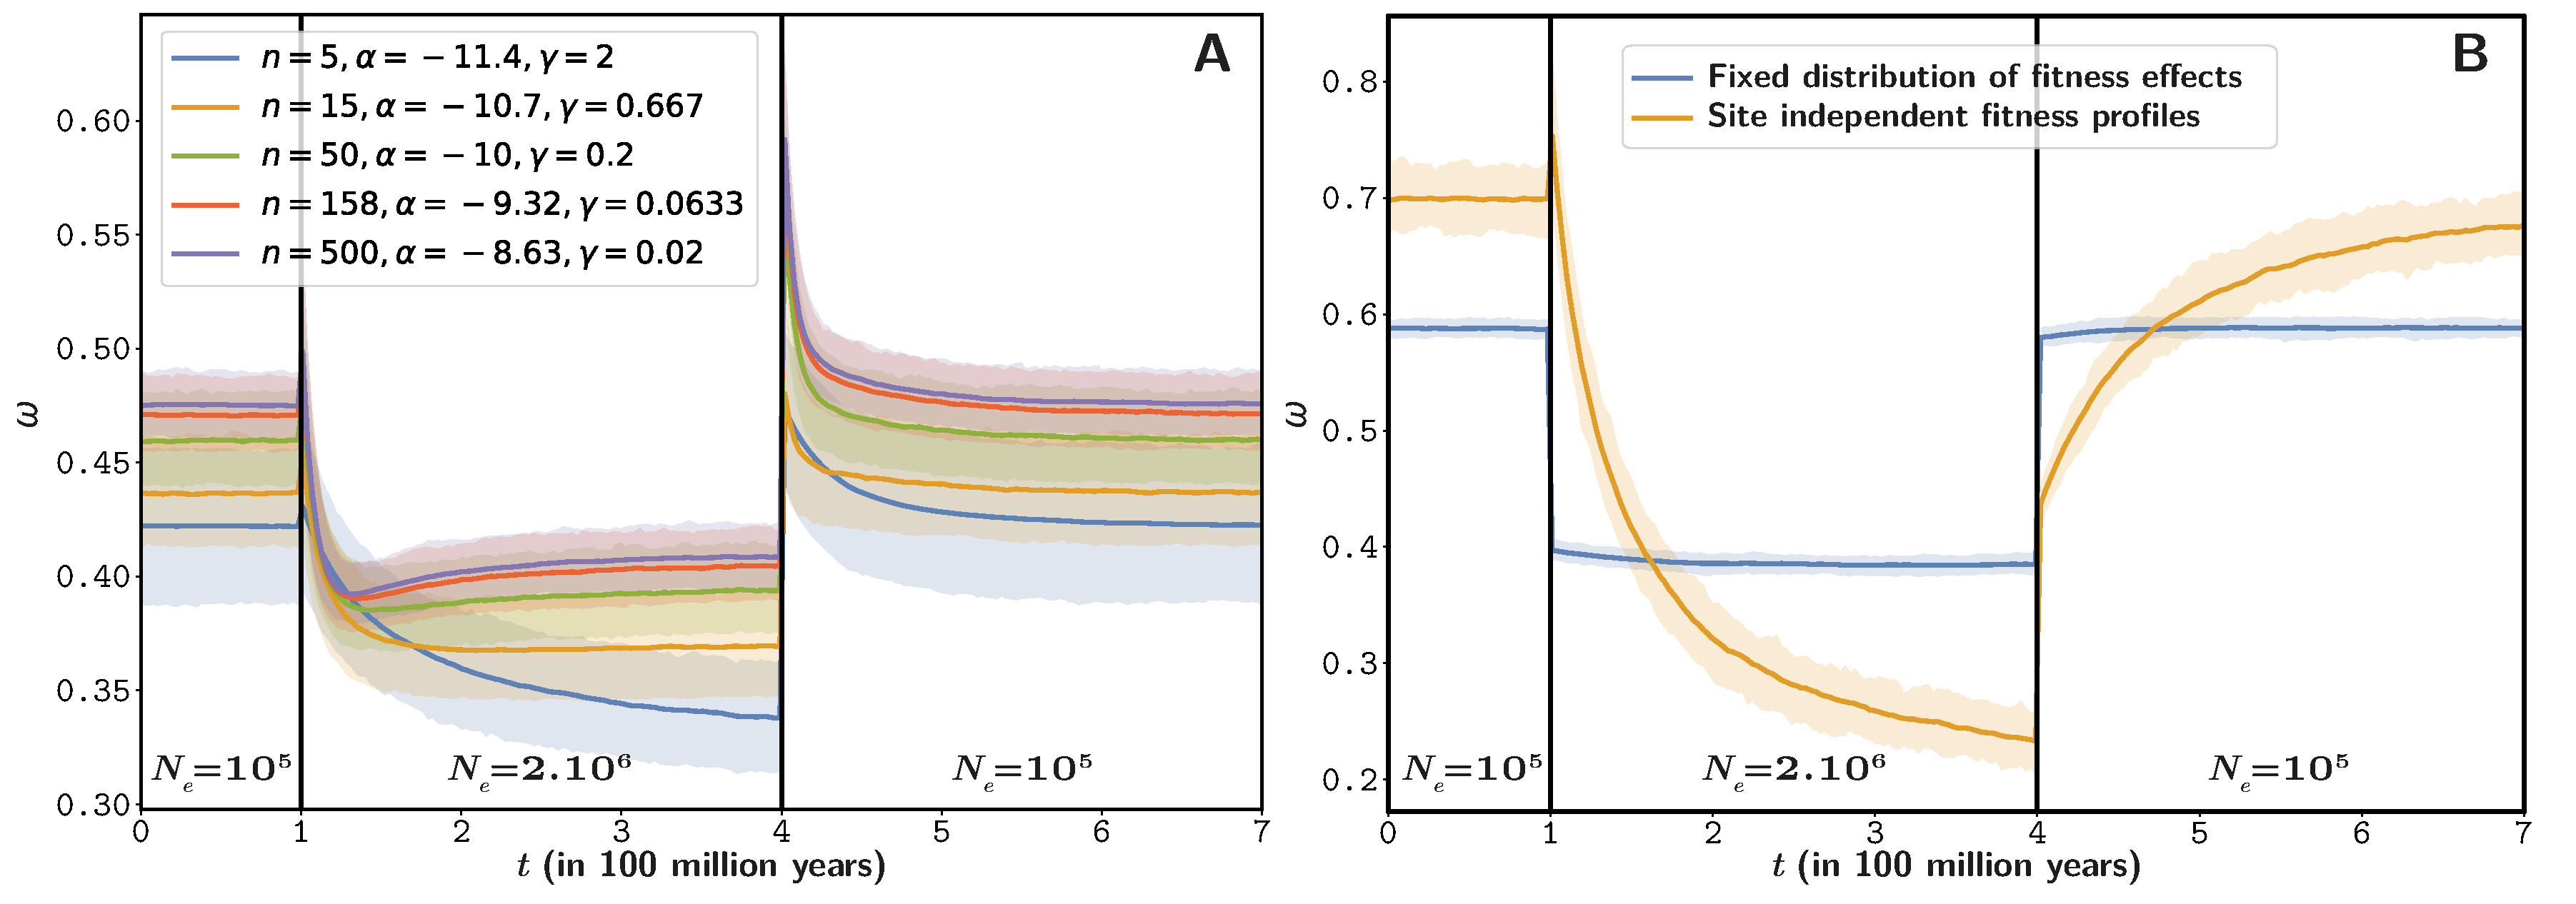
\includegraphics[width=0.9\textwidth] {artworks/Relaxation.pdf}
 \caption{
  \textbf{$\bm{\dnds}$ relaxation time to changes in $\bm{\Ne}$}.
  $\dnds$ relaxation after a brutal change in $\Ne$.
  Solid line corresponds to the average over replicates and the shaded area correspond to the $90\%$ interval among replicates. 
  The mutation rate ($\mu$) is $1e{-8}$ per year per site, and the total time of the computation is $700$ million years.
  Panel A. $\beta=1.686$, $\gamma=-10$ for all simulations. The number of sites is changed from $\Nsite=15$ to $\Nsite=158$, and the number of replicates ($r$) is changed accordingly such that the total number of sites ($\Nsite*r$) is kept constant.
  Moreover, $\gamma$ is changed according to $\Nsite$ such that the product $\gamma\Nsite$ is kept constant, thus the elasticity of the $\dnds$ to changes in $\Ne$ is kept constant.
  Finally, $\alpha$ is changed according to $\Nsite$ and $\gamma$ such that the equilibrium value $\x\eq$ is kept constant, by solving numerically equation \ref{eq:equilibrium}.
  Increasing $\Nsite$ implies a reduced time to reach the new equilibrium.
  Panel B. In context of a fixed fitness landscape, where each amino-acid has different fitness (site-specific profile), the time taken to reach the new equilibrium value of $\dnds$ after a change in $\Ne$ is long, such that relaxation rate is on the order of the mutation rate. In the context of a distribution of fitness effects, the relaxation time is non-existent.
 }
 \label{fig:relaxStability}
\end{mdframed}
\end{figure*}

\subsection*{Distribution of fitness effects}
DNA mutations changing a genotype can result in a change of phenotype, and ultimately a change in fitness.
From a specific genotype, all the possible mutations thus result in a distribution a phenotypic effect (DPE) and fitness effects (DFE).
The DPE and DFE are not known a priori, but are the resulting consequence of the mutation-selection-drift balance (see Figure \ref{fig:Distribution}).
Empirically, these distributions are of particular importance since they can be obtained experimentally or inferred with other data.
As an example, DFE can be inferred from polymorphism dataset \cite{Eyre-walker2007, Galtier2016}. 
Moreover, the distribution of $\deltadeltaG=\gamma \Nsite \dx$ of novel mutations can be obtained experimentally.
\begin{figure*}[htb!]
 \begin{mdframed}
  \centering
  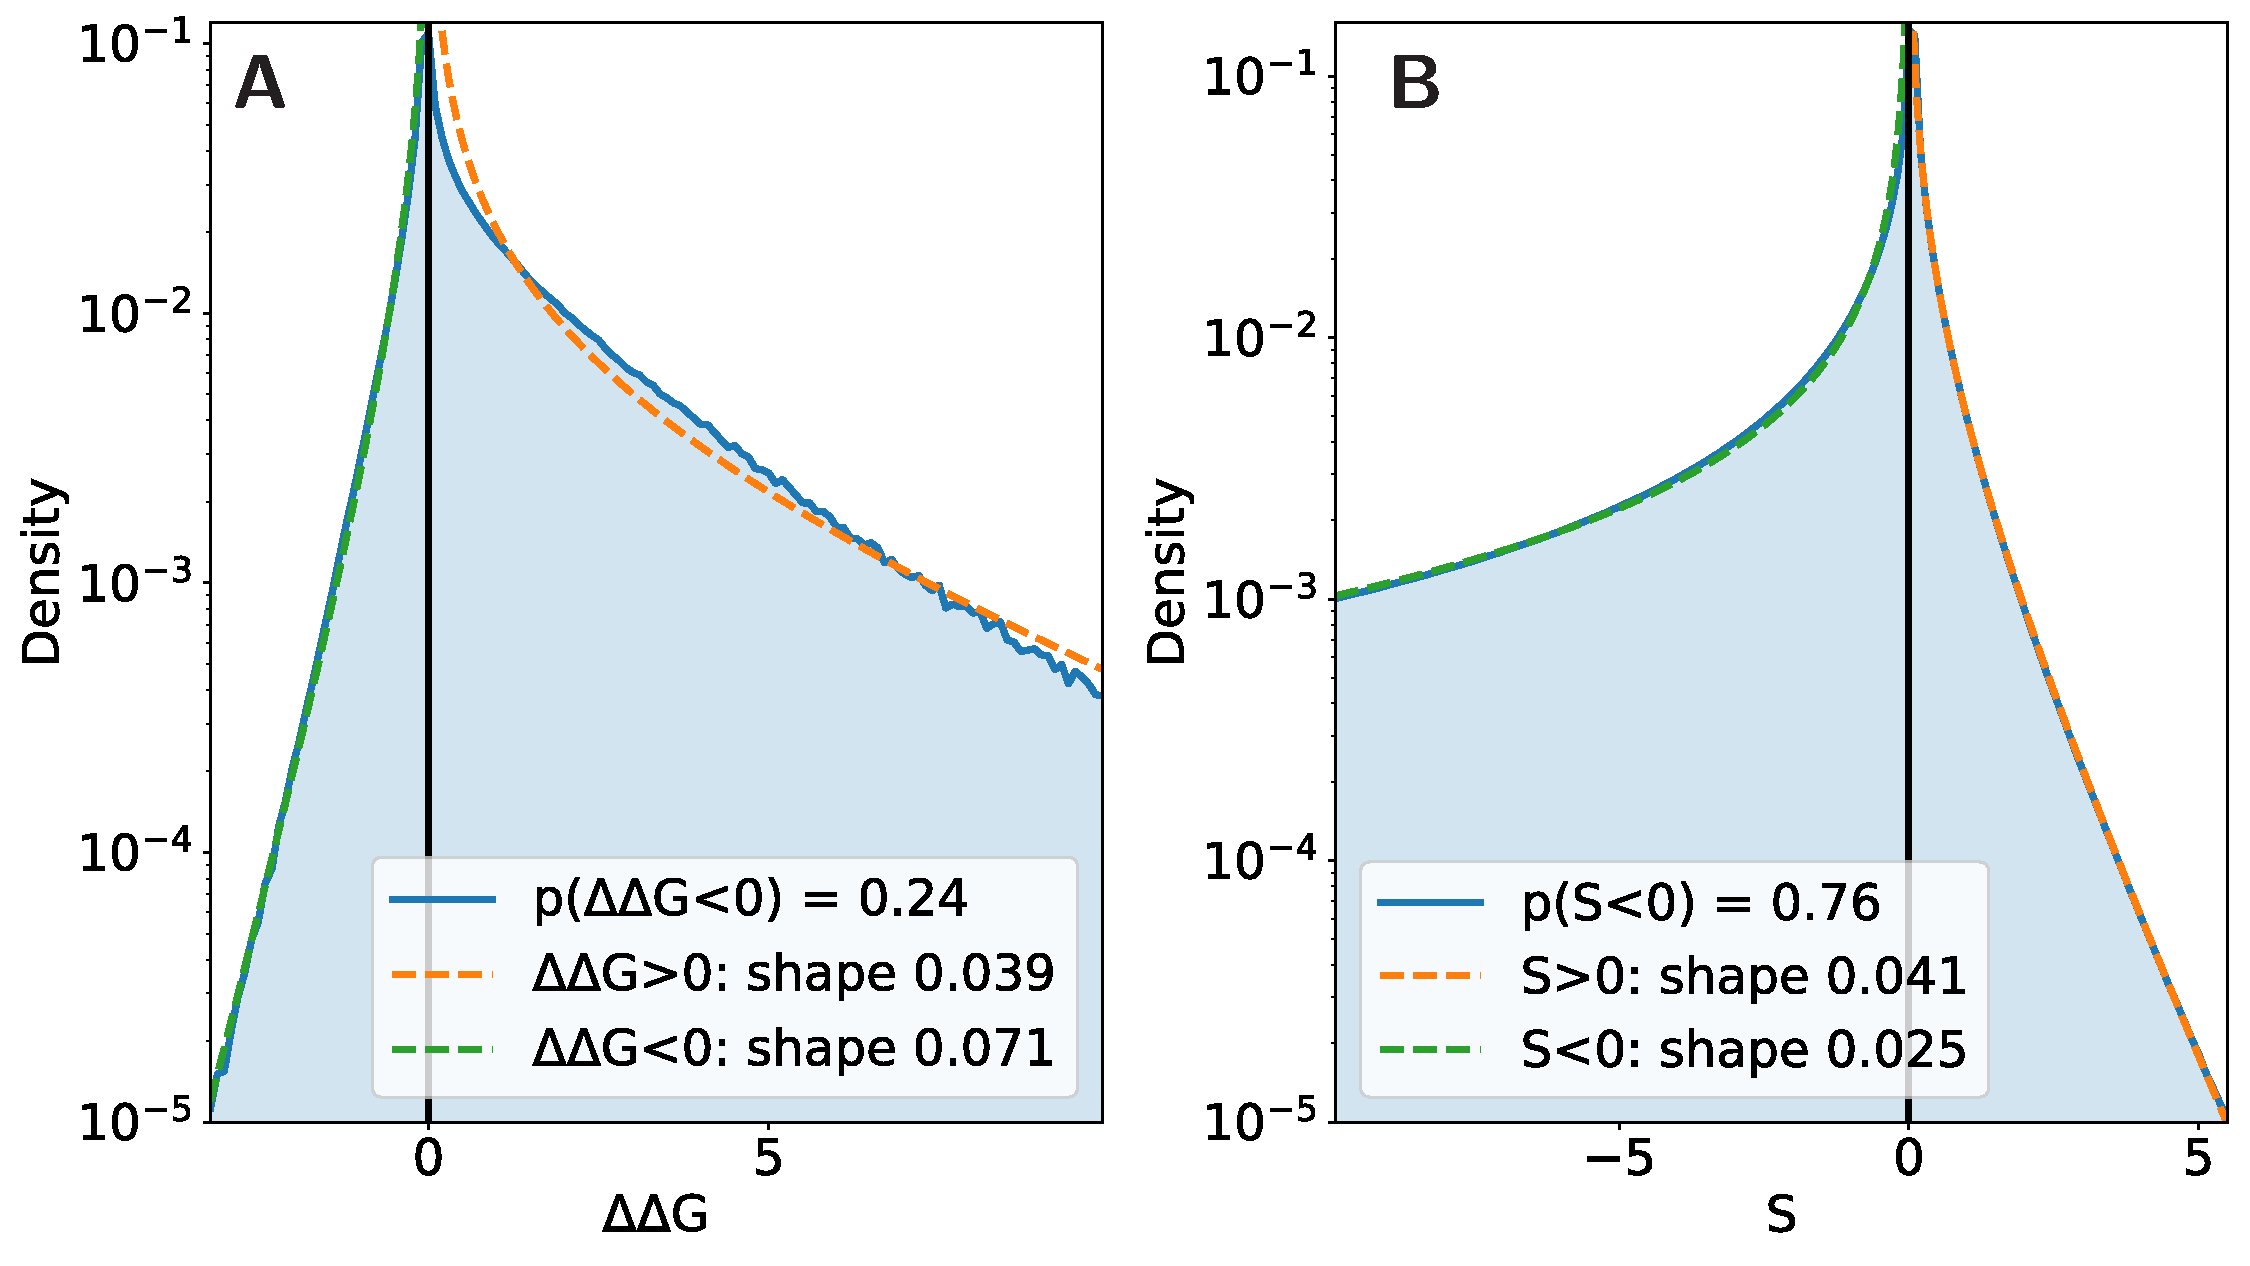
\includegraphics[width=0.9\textwidth] {artworks/DPE-DFE.pdf}
  \caption{
   \textbf{Distribution of phenotypic and fitness effects.}
   Distribution of fitness effects and phenotypic effect for novels non-synonymous mutations observed along a simulation at the mutation-selection balance. $\alpha=-118$, $\gamma=1$, $\Nsite=300$, $\beta=1.686$, and for each non-optimal amino-acid, $\gamma$ is scaled by the Grantham distance to the optimal amino-acid.
   Each side of the distribution is fitted to a gamma distribution, shown in dotted line. 
   Panel A. Distribution of observed $\deltadeltaG$, which fit adequately the gamma distribution for negative $\deltadeltaG$ (stabilizing mutations). 
   Panel A. Distribution of observed selection coefficient, which fit adequately the gamma distribution for both positive and negative selection coefficient. However the shape parameter estimated is not the same for positive and negative selection coefficients. 
  }
  \label{fig:Distribution}
 \end{mdframed}
\end{figure*}
\section*{Discussion}
Goldstein \& Pollock argued that model of protein evolution should consider how the acceptance of mutations depends on the sequence context in which they arise (epistasis), as to correctly represent resultant rate heterogeneity along the sequence, to predict the role of compensatory substitutions in protein evolution, predict which of the 10\% of deleterious mutations in humans are harmless in other species, or to accurately represent the rate and time dependence of convergence and homoplasy \cite{Goldstein2017}.
We argue that not taking into account epistasis also have the consequence of overestimating the relaxation time to return to equilibrium of $\dnds$ after changes in $\Ne$.
Paradoxically, not taking into account epistasis means overestimating the response of $\dnds$ to changes in $\Ne$ at equilibrium.\\
If using a distribution of fitness effect (DFE) is mathematically convenient and does not suffer from underestimating the relaxation rate, it is also overestimating the response of $\dnds$ to changes in $\Ne$ at equilibrium.
As such, developing inference of fitness landscape will require to assume site-interdependent fitness landscapes.\\
\section*{Materials \& Methods}
Protein sequence evolution is simulated under an origin-fixation model \cite{McCandlish2014}., where the rate of substitution of a new mutation with selection coefficient $s$ is:
\begin{equation}
p_{\text{fix}}(s) = \mu \dfrac{4 \Ne s}{1 + e^{- 4 \Ne s }}, 
\end{equation}
where $\mu$ is the mutation rate.
\subsection*{Simulation of protein folding with an additive model of free energy}
\label{MatMet:folding}
From a DNA sequence $\ci$ after $t$ substitutions, the protein's difference in free energy between folded and unfolded state is given by:
\begin{equation*}
\deltaG\left(\ci\right) = \deltaGMin + \Nsite \gamma * \x\left(\ci\right), 
\end{equation*}
where $\x\left(\ci\right)$ is the proportion of non-optimal amino-acid sites in the sequence.
Wrightian fitness is defined as the probability of our protein to be in the folded state, given by the Boltzmann equation: 
\begin{equation}
f(\deltaG\left(\ci\right)) = \dfrac{P_{\mathrm{F}}\left(\ci\right)}{P_{\mathrm{F}}\left(\ci\right) + P_{\mathrm{U}}\left(\ci\right)} = \dfrac{e^{-\beta G_{\mathrm{F}}\left(\ci\right) }}{e^{-\beta G_{\mathrm{F}} \left(\ci\right) } + e^{-\beta G_{\mathrm{U}}\left(\ci\right) }} = \dfrac{1}{1 + e^{\beta \deltaG\left(\ci\right) }}, 
\end{equation}
where $\beta$ is the inverse of the temperature ($\beta=1/kT$).
From the resident sequence $\ci$, we define $\setNeighbors$ as the set of all possible mutant that are one nucleotide away from $\ci$, and were mutant sequences containing a stop codon are excluded.
For a protein of $\Nsite$ amino-acid sites, $\left| \setNeighbors \right| \leq 9 \Nsite$, since each codon has a maximum of $9$ possible mutant codons that are one mutation away and that are not stop codon.
For each mutant sequence $\cj \in \setNeighbors$, we compute $\deltaG^{t+1}$ from the updated sequence $\cj$, and subsequently the selection coefficient of the mutant:
\begin{equation}
s \left( \ci,\cj\right) = \dfrac{ f\left( \deltaG \left(\cj\right) \right) - f\left( \deltaG \left(\ci\right) \right)}{f\left( \deltaG \left(\ci\right) \right)}.
\end{equation}
The next change in the protein-coding DNA and the time to next the event is chosen using Gillespie algorithm, according to the rates of substitution between codons:
\begin{equation}
\submatrix_{\itoj} = \mu_{\itoj} \dfrac{4 \Ne s \left( \ci,\cj\right)}{1 - \e^{-4 \Ne s \left( \ci,\cj\right)}}, 
\end{equation}
where $\mu_{\itoj}$ is the mutation rate between $\ci$ and $\cj$, determined by the underlying $4x4$ nucleotide mutation rate matrix, and ${\submatrix_{\itoj}} = \mu_{\itoj}$ in the case of synonymous substitutions.
\subsection*{Simulation with independent fitness profiles}
A fitness profile give a fitness for each amino-acid (vector of size $20$).
Each site of the protein has a specific amino-acid fitness profile.
Overall, the protein phenotype is computed as the sum of site-specific selection coefficient, obtained by accessing the amino-acid present at each site of the protein.
The selection coefficient of the mutant $\cj$ is:
\begin{equation}
s \left( \ci,\cj\right) = \sum_{1 \leq \site \leq \Nsite} \ln \left( \dfrac{G_{\site} \left(\cj(\site) \right)}{G_{\site} \left(\ci(\site) \right)} \right) ,
\end{equation}
where $G_{\site}$ is the fitness profile at site $\site$, obtained in empirical experiment \cite{Bloom2017}.
The next change in the protein-coding DNA and the time to next the event is chosen using Gillespie algorithm, as in \ref{MatMet:folding}.
\subsection*{Simulation with distribution of fitness effects (DFE)}
The selection coefficient of the mutant $\cj$ is gamma distributed (shape $\beta > 0$):
\begin{equation}
- s \left( \ci,\cj\right) \sim \text{Gamma} \left( \bar{|s|}, \beta \right)
\end{equation}
The next change in the protein-coding DNA and the time to next the event is chosen using Gillespie algorithm, as in \ref{MatMet:folding}.
\subsection*{$\bm{\dnds}$ along the simulation}
From the set of mutants $\setNeighbors$ that is one nucleotide away from $\ci$, we define the subsets $\setNonSynNeighbors$ and $\setSynNeighbors$ that are respectively the set of non-synonymous and synonymous mutants, where $\setNonSynNeighbors \cup \setSynNeighbors = \setNeighbors$.
As in previous works \cite{Spielman2015a, DosReis2015, Jones2016}, the ratio of non-synonymous over synonymous substitution rates of the sequence is defined as :
\begin{align}
\dnds(t) &= \dfrac{\sum_{\cj \in \setNonSynNeighbors} \submatrix_{\itoj}}{\sum_{\cj \in \setNonSynNeighbors} \mu_{\itoj}} \left( \dfrac{\sum_{\cj \in \setSynNeighbors} \submatrix_{\itoj}}{\sum_{\cj \in \setSynNeighbors} \mu_{\itoj}} \right)^{-1}\\
 &= \dfrac{\sum_{\cj \in \setNonSynNeighbors} \mu_{\itoj} \dfrac{4 \Ne s \left( \ci,\cj\right)}{{1 - \e^{-4 \Ne \left( \ci,\cj\right)} }}}{\sum_{\cj \in \setNonSynNeighbors} \mu_{\itoj}} 
\end{align}
\subsection*{Reproducibility}
The simulators written in C++ are publicly available under MIT license at \url{https://github.com/ThibaultLatrille/SimuEvol}.
The scripts and instructions necessary to reproduce the experiments are available at \url{https://github.com/ThibaultLatrille/GenotypePhenotypeFitness}.
\bibliographystyle{apalike}
\bibliography{refs-codons,refs-cds}

\end{document}